\documentclass[]{article}

\usepackage[utf8]{inputenc}

\usepackage{eurosym}
\usepackage[
  margin=1.8cm,
  includefoot,
  footskip=10pt,
]{geometry}
\usepackage{graphicx}
\graphicspath{{figures/}}
\usepackage[english]{babel}
\usepackage{url}
\usepackage[colorlinks=true, linkcolor=black, urlcolor=blue]{hyperref}
\usepackage{color}
\usepackage[dvipsnames]{xcolor}
\usepackage{titling}
\usepackage{subfig}
\usepackage[bottom]{footmisc}
\usepackage{titlesec}
\usepackage{chngpage}
\usepackage{calc}
\usepackage{listings}

\definecolor{gray}{rgb}{0.4,0.4,0.4}
\definecolor{darkblue}{rgb}{0.0,0.0,0.6}
\definecolor{cyan}{rgb}{0.0,0.6,0.6}

\lstset{
  basicstyle=\ttfamily,
  columns=fullflexible,
  showstringspaces=false,
  commentstyle=\color{gray}\upshape
}


\setcounter{secnumdepth}{4}


\newcommand{\minit}[1]{\noindent{\small\textbf{ \underline{#1}}}~\\}
\newcommand{\todo}[1]{\par{\color{red} /---| A faire : #1 |---\textbackslash\\}}
\newcommand{\todoIL}[1]{{\color{red}[todo: #1]}}
\newcommand{\wordlink}[2]{\hyperref[#2]{#1~\ref{#2}}}

\titleformat{\paragraph}
{\normalfont\normalsize\bfseries}{\theparagraph}{1em}{}
\titlespacing*{\paragraph}
{0pt}{3.25ex plus 1ex minus .2ex}{1.5ex plus .2ex}

%-- Logos PDG --
\pretitle{
\begin{center}

\begin{figure}[!tbp]
  \centering
  \subfloat{
\includegraphics[width=0.25\textwidth]{UMons_logo.png}}
  \hfill
  \subfloat{
\includegraphics[width=0.25\textwidth]{sciences_logo.png}}\\
\end{figure}
~\newline

}

\posttitle{\end{center}}

\begin{document}

\title{
\vspace{1.6cm}
{\Huge Software Analysis : pacman systems}\\
\vspace{0.5cm}
{\Huge Project report for Software Evolution course}\vspace{1cm}\\
}


\author{
\vspace{1cm}
\huge{Group 3}\\
\Large{BOOSKO Sam}\\
\Large{DECOCQ Rémy}\\
\Large{SCHERER Robin}
}


\date{
\vspace{7.9cm}
Academic Year 2019-2020\\
Master Computers Science, block 2\\
Faculté des Sciences, Université de Mons}

\maketitle          

\thispagestyle{empty}   

\newpage

\tableofcontents
\newpage

%------------- INTRO -------------
\section*{Introduction}
\newpage
\section{Quality analysis of the initial versions}
\label{quality_analysis}

\subsection{System 2 (Rémy)}
\subsubsection{Generalities}

First of all, this is noticeable that authors provide some documents coupled with the implementation, even if it is not mentioned in the README file. This additional material is available under the \texttt{out/} directory at project roots and comprises :
\vspace{0.1cm}
\begin{itemize}
\item A \texttt{.pdf} file describing shortly the game, the controls and the multiplayer (2 players) mode available

\item A complete class diagram covering the whole implementation

\item A sequence diagram stating the execution flow when Pacman arrives on a cell and so ``eat" what is at this place

\item A graph of the mathematical function used to correlate difficulty with player's progression
\end{itemize}

We also observe that in this Pacman implementation maps are modelized under \texttt{.tmx} format, that is a popular way to deal with board games\footnote{\url{https://doc.mapeditor.org/en/stable/reference/support-for-tmx-maps/}}. Only one single basic map is provided.\\

The project structure is classic, we have \texttt{main} and \texttt{test} separation under the \texttt{src} directory, each containing packaged sources. The building system provided with the implementation is hold by Gradle. So a switch to Maven will be required to comply with directives.


\subsubsection{Static Analysis}

\paragraph{Code metrics (CodeMR)}

CodeMR allows to get an overall idea of the actual health of the system considering several metrics. The dashboard illustrated by \wordlink{Figure}{fig:S2_codeMR_dashboard} informs this software is doing quite good.

\begin{figure}[h]
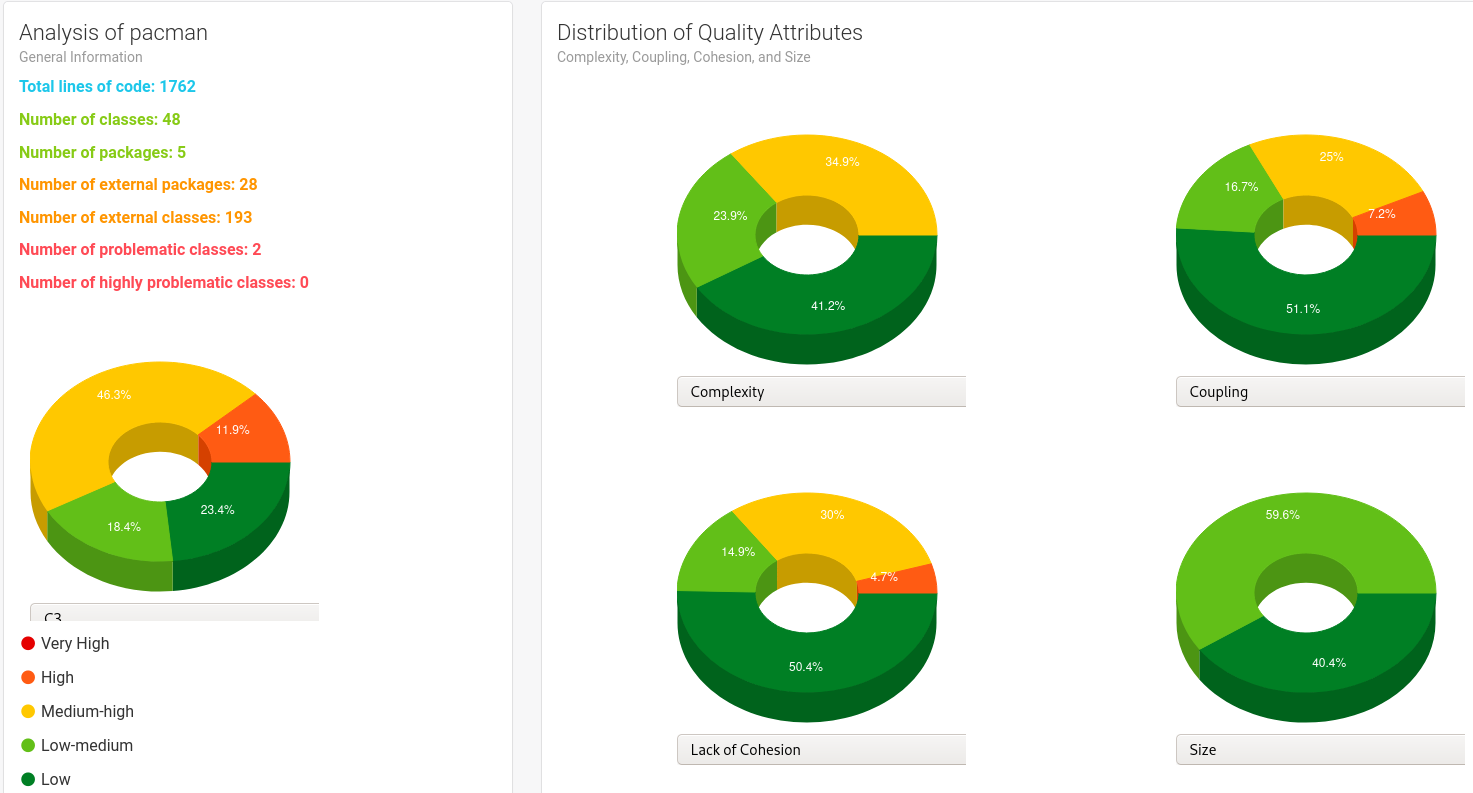
\includegraphics[width=\linewidth]{S2-codeMR_dashboard}
\caption{CodeMR dashboard summarizing health of system 2}
\label{fig:S2_codeMR_dashboard}
\end{figure}

\newpage

The \wordlink{Figure}{fig:S2_codeMR_packages} illustrates also the C3 metric but coupled with detailed packages view. We notice authors apparently tried to follow some Model-View-Controller pattern to design their application. The C3 metric is defined as the maximum between 3 other well representative metrics : \textit{Coupling}, \textit{Cohesion} and \textit{Complexity}. These are defined in the codeMR documentation\footnote{\url{https://www.codemr.co.uk/documents}}. We notice that, following the dashboard overview, two classes are impacting the software quality from the point of view of C3 metric.
\vspace{0.2cm}
\begin{figure}[h]
\centering
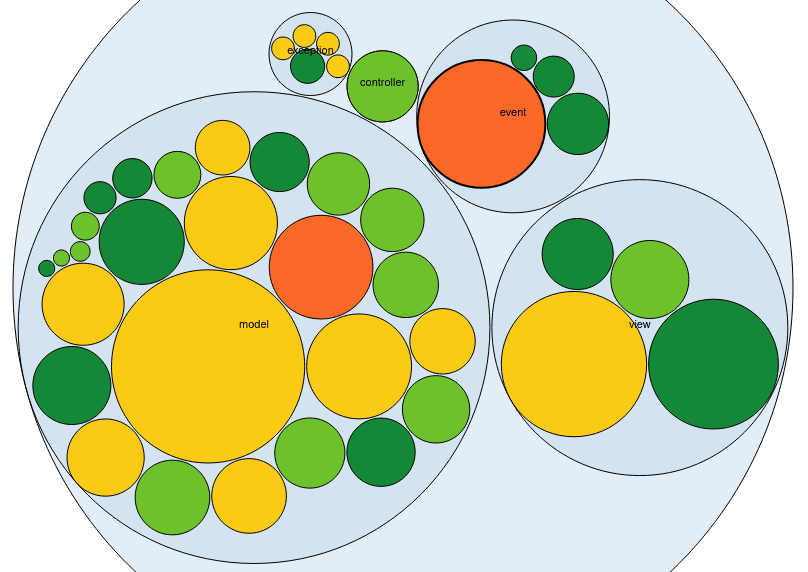
\includegraphics[width=0.8\linewidth]{S2-codeMR_packages}
\caption{C3 Metric by package for system 2}
\label{fig:S2_codeMR_packages}
\end{figure}

The details of the measurements on the two more problematic classes are given by \wordlink{Figure}{fig:S2_workerProcess} and \wordlink{Figure}{fig:S2_ghost}, for respectively \textit{event.WorkerProcess} and \textit{model.Ghost}. For both, two metrics are considered as high value, the meaning described by CodeMR is
\begin{itemize}
\item LTCC : The Lack of Tight Class Cohesion metric measures the lack cohesion between the public methods of a class. That is the relative number of directly connected public methods in the class. Classes having a high lack of cohesion indicate errors in the design.
\item LCOM : Measure how methods of a class are related to each other. Low cohesion means that the class implements more than one responsibility. A change request by either a bug or a new feature, on one of these responsibilities will result change of that class. Lack of cohesion also influences understandability and implies classes should probably be split into two or more subclasses.
\end{itemize}

In addition, for \textit{event.WorkerProcess} we have :
\begin{itemize}
\item CBO : The number of classes that a class is coupled to. It is calculated by counting other classes whose attributes or methods are used by a class, plus those that use the attributes or methods of the given class.
\item AFTD : Access to Foreign Data is the number of classes whose attributes are directly or indirectly reachable from the investiggated class. Classes with a high ATFD value rely strongly on data of other classes and that can be the sign of the God Class.
\end{itemize}

Other codeMR metrics did not revelate relevant problems in the implementation.

\newpage

\begin{figure}[h]
\centering
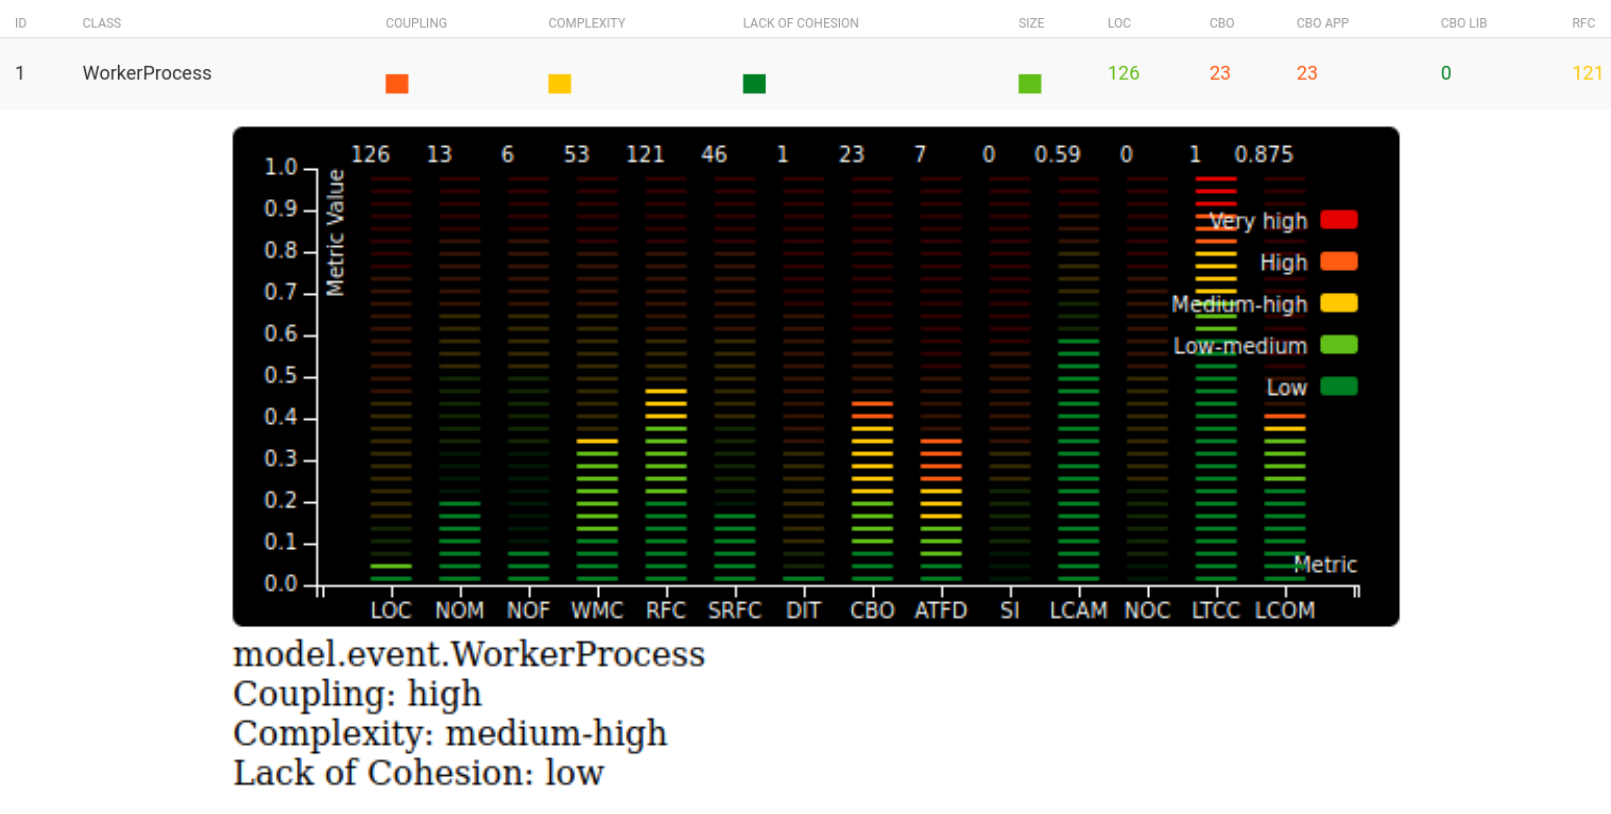
\includegraphics[width=0.9\linewidth]{S2-WorkerProcess_full}
\caption{\textit{event.WorkerProcess} class main metrics measurements}
\label{fig:S2_workerProcess}
\end{figure}

\begin{figure}[h]
\centering
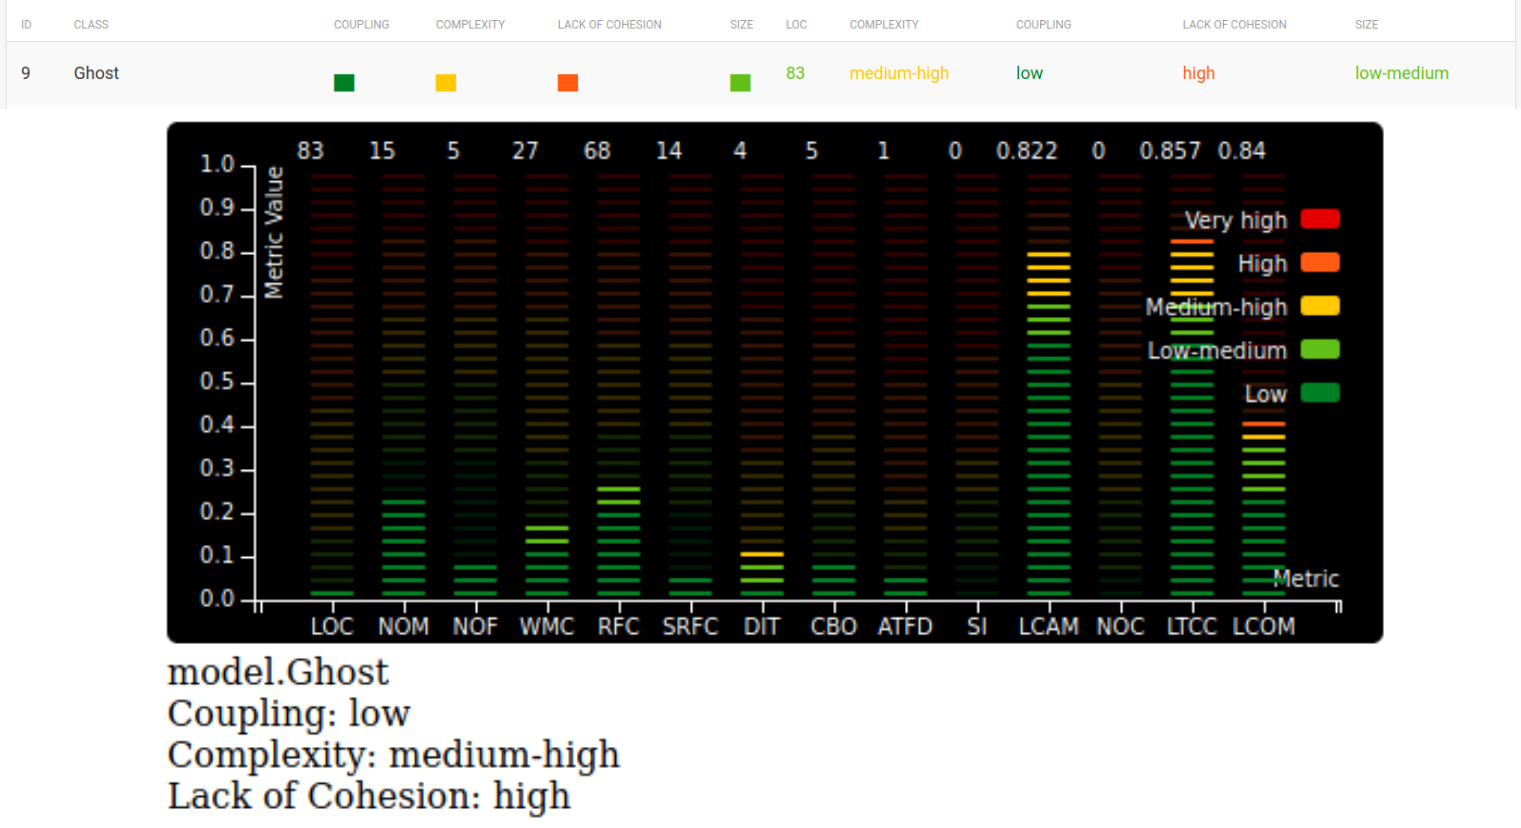
\includegraphics[width=0.82\linewidth]{S2-Ghost_full}
\caption{\textit{model.Ghost} class main metrics measurements}
\label{fig:S2_ghost}
\end{figure}
  
\newpage

\paragraph{Dependencies (CodeMR, Intellij analyzer)}

CodeMR allows also to inspect dependency relations between classes coupled with the metrics measured for each. We observe in the \wordlink{Figure}{fig:S2_inheritance} the same structure that in the class diagram. Once again the class \textit{event.WorkerProcess} is displayed as problematic, being too complex and coupled with other classes.\\

We use the standard built-in tool of IntellIJ IDEA to instantiate the dependency matrix, illustrated by \wordlink{Figure}{fig:S2_dep_matrix}. We clearly see reading 8th column that \textit{event.WorkerProcess} depends on a lot of other classes from package \textit{model}. This is also the case for \textit{model.Map} that presents a lot of cyclic dependencies (red marked).

\paragraph{Compliance \& bad smells (PMD, Designite)}

PMD is a statical analyzer that checks for problems of several natures in the code. It detected more than 1500 violations in the system 2, related to various topics (see \wordlink{Figure}{fig:S2_PMD}).

\vspace{0.3cm}

\begin{figure}[h]
\centering
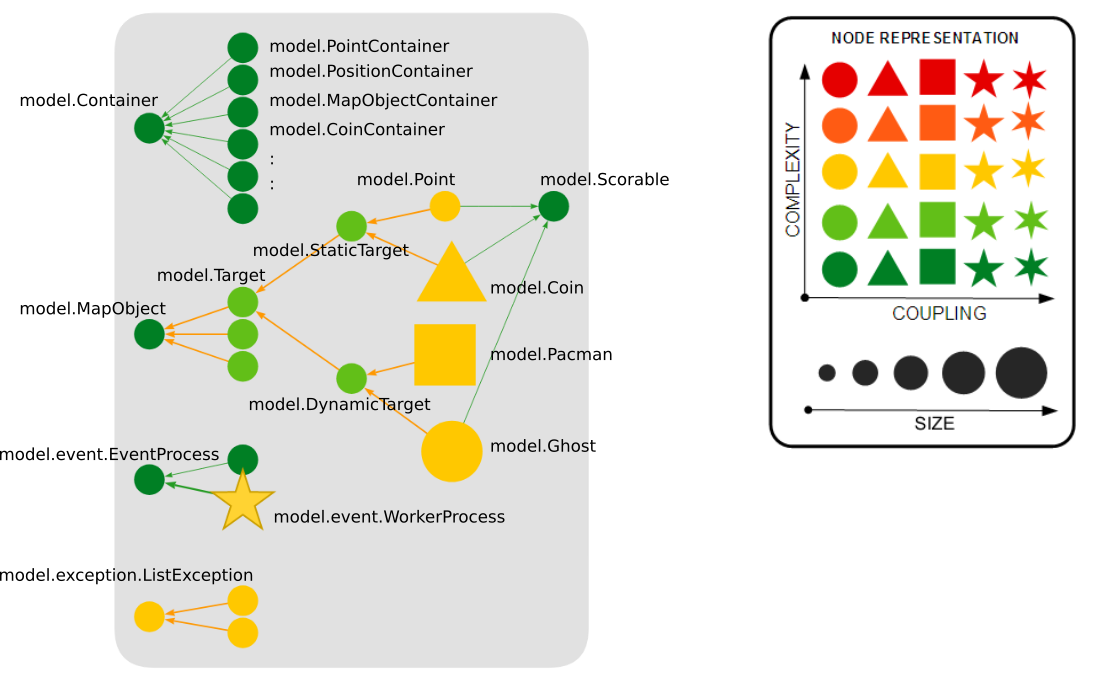
\includegraphics[width=0.8\linewidth]{S2-named_inheritance}
\caption{Inheritance relations between classes in system 2}
\label{fig:S2_inheritance}
\end{figure}

\vspace{0.4cm}

\begin{figure}[h]
\centering
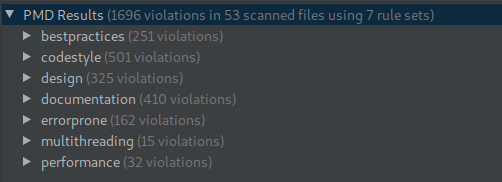
\includegraphics[width=0.7\linewidth]{S2-PMD_results}
\caption{Violations found by PMD in system 2}
\label{fig:S2_PMD}
\end{figure}

\newpage

\begin{figure}[h]
\centering
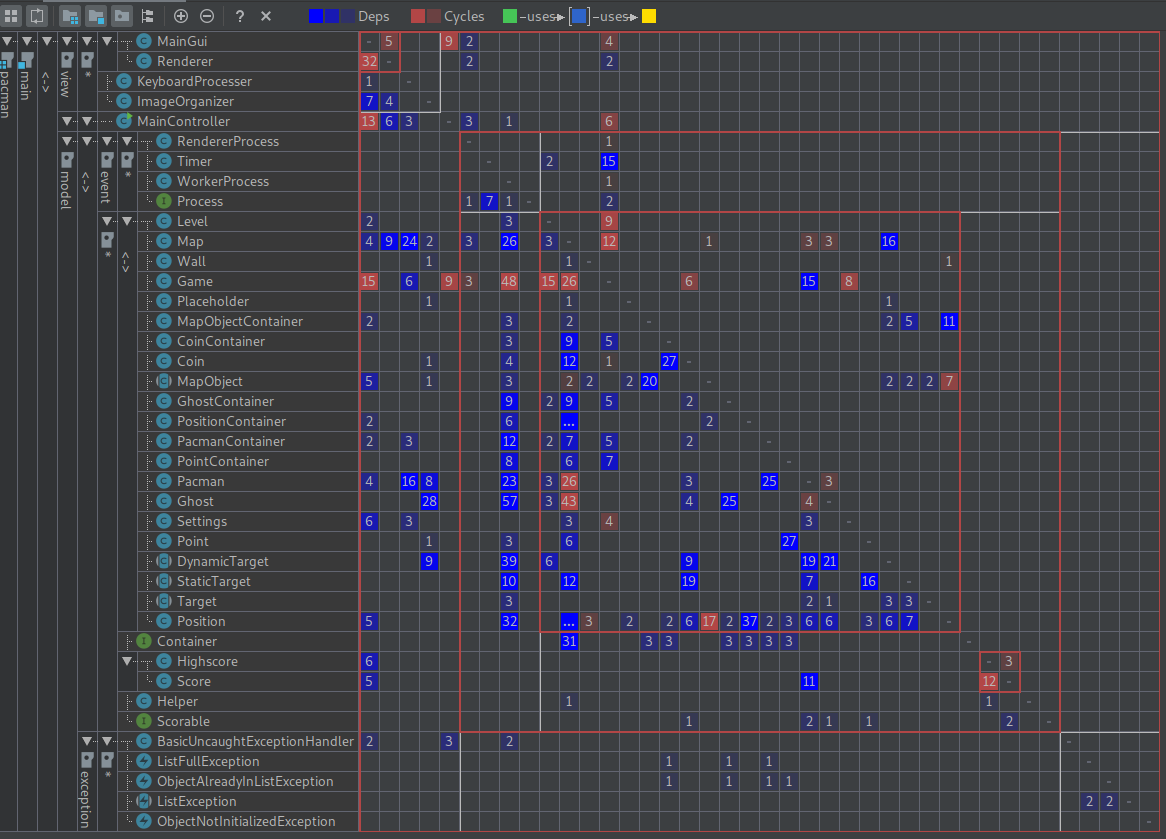
\includegraphics[width=0.9\linewidth]{S2-dep_matrix}
\caption{Dependency matrix for system 2}
\label{fig:S2_dep_matrix}
\end{figure}

\vspace{0.1cm}

Designite is used to detect bad smells, a summary of the analyse is presented by \wordlink{Figure}{fig:S2_designite}. The number of lines of code and classes is higher than the ones returned by CodeMR because the test sources were considered in the analysis.

\begin{figure}[h]
\centering
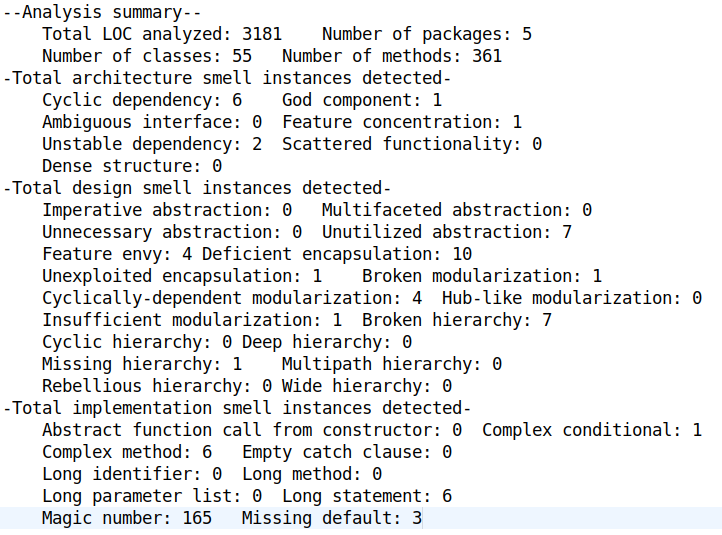
\includegraphics[width=0.65\linewidth]{S2-designite}
\caption{Designite in-line use results for system 2}
\label{fig:S2_designite}
\end{figure}


\newpage


\paragraph{Javadoc coverage (MetricsReloaded)}

We use the IntellIJ MetricsReloaded plugin and its metric "Javadoc coverage" to get an overview of how complete is the initial javadoc. As shown by \wordlink{Figure}{}, this is the case.

\vspace{0.2cm}

\begin{figure}[h]
\centering
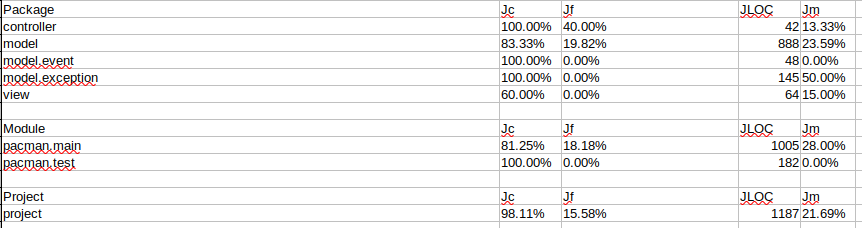
\includegraphics[width=0.65\linewidth]{S2-javadoc}
\caption{Javadoc coverage for system 2}
\label{fig:S2_javadoc}
\end{figure}

\subsubsection{Dynamic Analysis}

\paragraph{Running tests}

Among the already written tests, 3 out of 67 failed at running time. The three tests are in \textit{model.LevelTest} (\textit{testGetLevel}, \textit{testSecondsForCoin} and \textit{testNextLevel}). 

\paragraph{Test coverage (Intellij built-in tool)}

IntellIJ provides run configurations to dynamically analyze what are the parts of source codes covered by launched tests. Considering whole test packages, summary of the results are given by \wordlink{Figure}{fig:S2_test_coverage}. We observe the implementation benefits of a good test coverage, the most laking part is package \textit{view} but it makes sense by its nature.

\newpage

\begin{figure}[h]
\centering
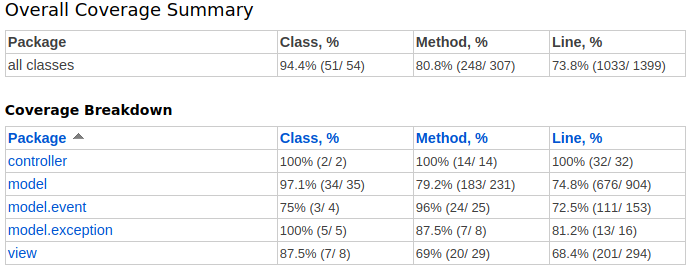
\includegraphics[width=0.75\linewidth]{S2-test_coverage}
\caption{Test coverage for system 2}
\label{fig:S2_test_coverage}
\end{figure}

\newpage
\section{Quality improvement}

\subsection{System 2 (Rémy)}

We employ the following methodology to improve the system in its current state :
\begin{enumerate}
\item Reviewing the whole code and correct problems of form. It allows to acquire a global overview of the implementation to lead next steps and improve code quality on a per-class basis. These refractorings comprise, among others :
\begin{itemize}
\item completing the Javadoc
\item getting rid of forgot/useless artifacts
\item detecting and correcting code smells
\end{itemize}
The main tool used during this step will be the IDE (IntellIJ) and plugins associated with like Designite, which allow on-the-fly analysis and pointing out problems in the code itself.


\item Reviewing the system structure and correct structural design problems. From the acquired global overview, it is possible to have an idea of drawbacks implied by the system design. The refractoring will occurr at a class-to-class relations level, and will then impact package structure level. Some tools and metrics, for example from CodeMR, can be used to leas this step : a class reported too long may be splitted into more than 1 class, inheritance should be used better, etc.

\item If some tests are not passing, find the reason and correct them.

\item Complete the tests based on test coverage reports generated (from IntellIJ).

\item Reuse all the same tools than in \wordlink{Section}{quality_analysis} to generate new reports and observe how quality variated.
 
\end{enumerate}
\vspace{0.2cm}
Of course, after each of these steps, the current yet written tests must be launched to control the consistence of the implementation.

\subsubsection{Step 1}

We read through the whole code and corrected what had to be in a first time. Some smells are straightforward, like avoiding Magic Numbers detected by Designite. The help of IntellIJ is precious to get rid of some deprecated/forgot code artifacts the authors left. Some problems reported by Designite are not regarding the actual usage and left as-is.

\subsubsection{Step 2}

It was figured out the current implementation presents some drawbacks. It is mainly related to code duplication for already written objects for \texttt{Container} purposes (can be found in provided class diagram). The fact is that authors wanted to write an overlayer to describe different collections of other objects in the implementation (\texttt{Coin} (= pills), \texttt{Point}, etc.). But they wrote a specific class for every type of object to contain, albeit implementing the common \texttt{Container} interface, this design is very poor and ineleguant, leading to code duplication and increased number of classes. Keeping in mind what were each class written for, we redisigned this part of the implementation in a better way. It also brought the occasion to cluster \texttt{Container} class concerned in a new package to improve the project structure readability.\\

The resulting structure is depicted by \wordlink{Figure}{fig:S2_containers}. We now consider to pass through a \texttt{Containers} class to construct any \texttt{Container} needed in the rest of the implementation. Its methods instantiate the right container with adapted type from generic classes. These instances are shown in orange in the \wordlink{Figure}{fig:S2_containers}. A \texttt{PositionContainer} is a special container to hold coordinates, so we dont use an index but form a key from the couple ($x$, $y$).The method \texttt{getRange(..)} allow to get a subset of contained positions, considering a rectangle selection formed from two positions. For some object types (\texttt{Point}), an overload is necessary to comply with the rest of the implementation. Anyway, this is somehow masked because all containers instances are retrieved from the class \texttt{Containers} mentioned above, and not represented in the figure.

\newpage

\begin{figure}[h]
\centering
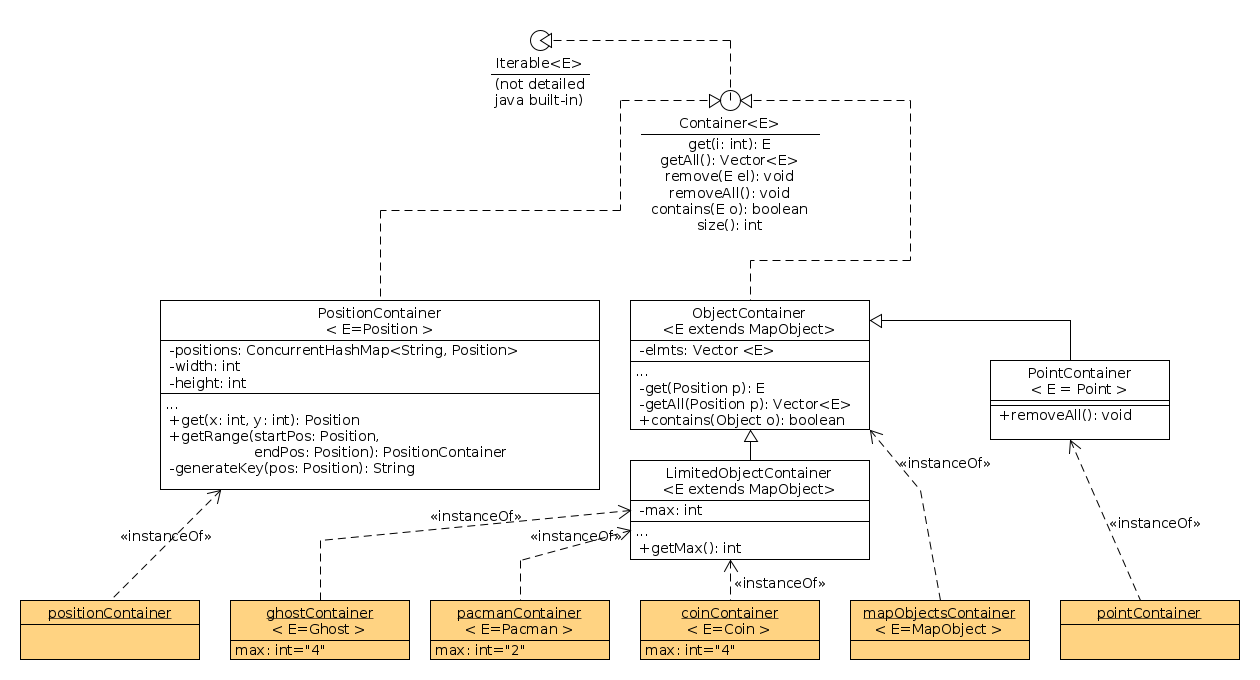
\includegraphics[width=\linewidth]{S2-classdiagram_containers}
\caption{New class structure for \texttt{Container}s part of the implementation}
\label{fig:S2_containers}
\end{figure}


\newpage
\section{Adding basic functionalities}
\newpage
\section{Adding new features}
\newpage
\section{Quality evolution analysis}
\newpage
\section{Conclusion}


\end{document}